\documentclass[]{article}
\usepackage{amsmath}
\usepackage{amssymb}
\usepackage{graphicx}
\usepackage{subfig}
\usepackage[newfloat]{minted}
\usepackage{caption}
\newenvironment{code}{\captionsetup{type=listing}}{}
\SetupFloatingEnvironment{listing}{name=Snippet}
\graphicspath{{./imgs/}}
%opening
\title{Normalizing Flows}
\author{Abdul Fatir}
\date{}
\begin{document}

\maketitle

\begin{abstract}
Notes on normalizing flows.
\end{abstract}
\subsection{Code for PReLU}
\begin{code}
	\inputminted[linenos=true,frame=lines,framesep=2mm]{python}{prelu.py}
	\captionof{listing}{Parametrized ReLU Bijector}
\end{code}
\subsection{Reproducing Results from Rezende and Mohamed}
Reproducibility is an important concern in deep learning, especially because the models are trained stochastically in environments that can be very different from each other.  With this is mind, and a lack of official implementation from the authors, I implemented planar flows and conducted a few experiments presented in the paper. 

The experiment seeks to approximate two complex 2D densities using planar flows. The unnormalized density functions are given by $p(\mathbf{z}) \propto e^{-U_i(\mathbf{z})}$ where the two energy functions $U_1$ and $U_2$ are
\begin{align}
U_1(\mathbf{z}) &= \frac{1}{2}\left(\frac{\|\mathbf{z}\| - 4}{0.4}\right)^2 - \log \left(e^{-\frac{1}{2}\left[\frac{z_1-2}{0.8}\right]^2} + e^{-\frac{1}{2}\left[\frac{z_1+2}{0.8}\right]^2} \right)\\
U_2(\mathbf{z}) &= \frac{1}{2}\left[\frac{z_2 - \sin\left(\frac{2\pi z_1}{4}\right)}{0.4}\right]^2
\end{align}

\begin{figure}
	\centering
	\subfloat[Density 1]{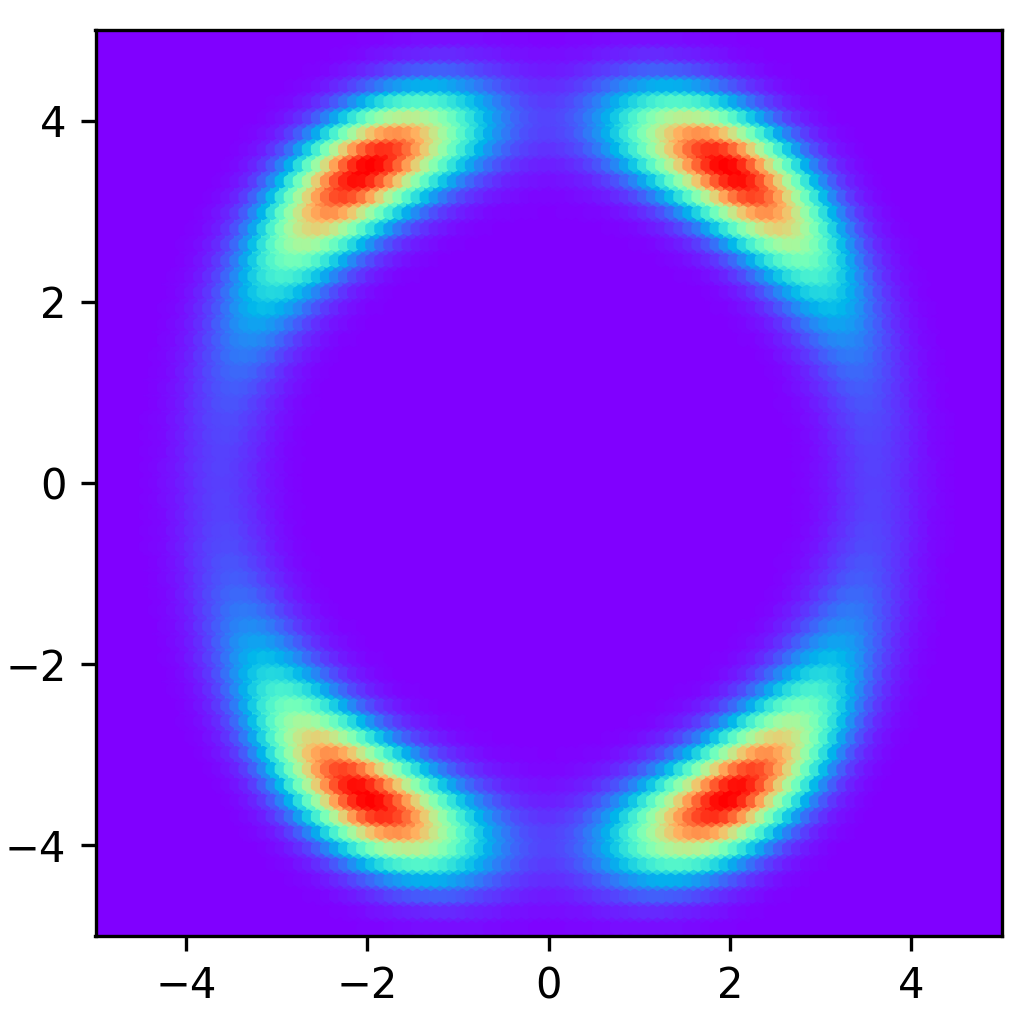
\includegraphics[width=0.5\textwidth]{example1-density}}
	\subfloat[Samples from Density 1]{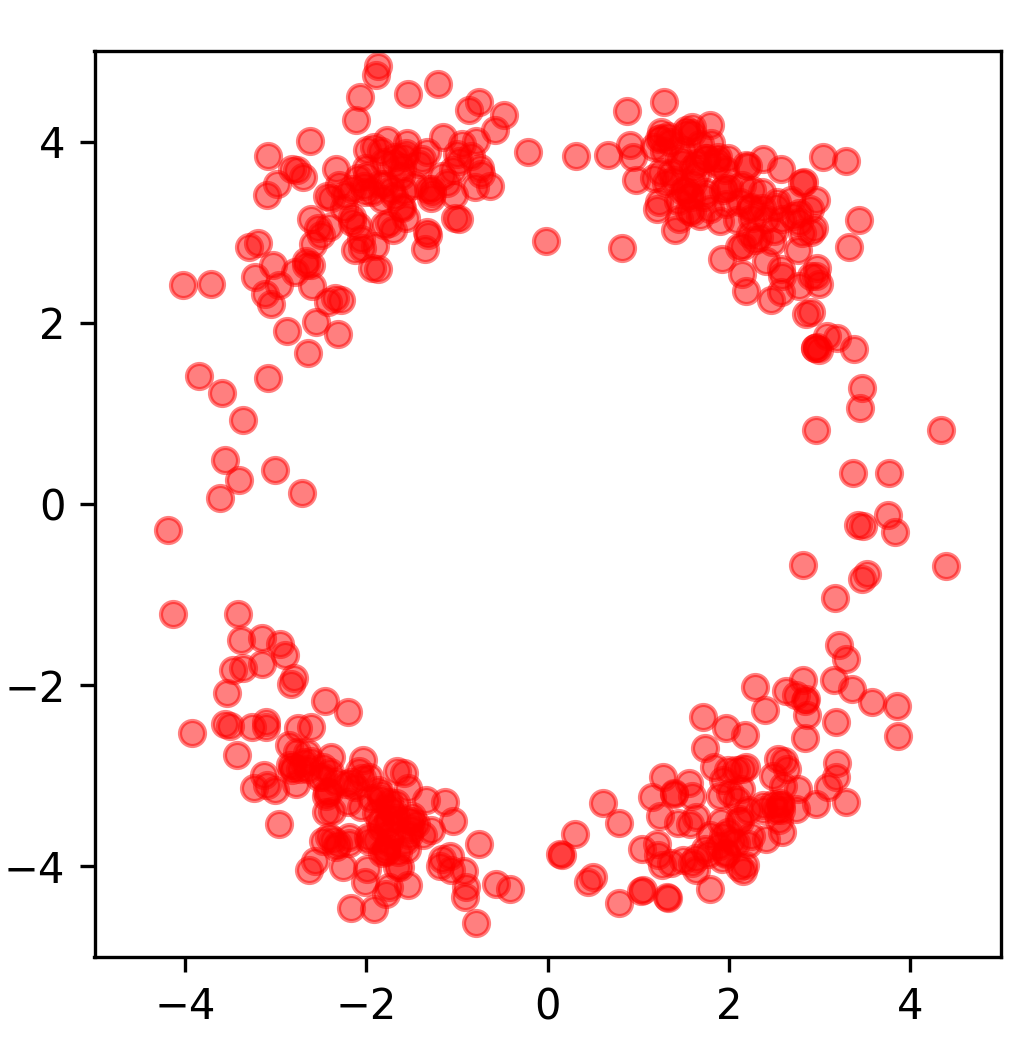
\includegraphics[width=0.5\textwidth]{example1-samples}}\\
	\subfloat[Density 2]{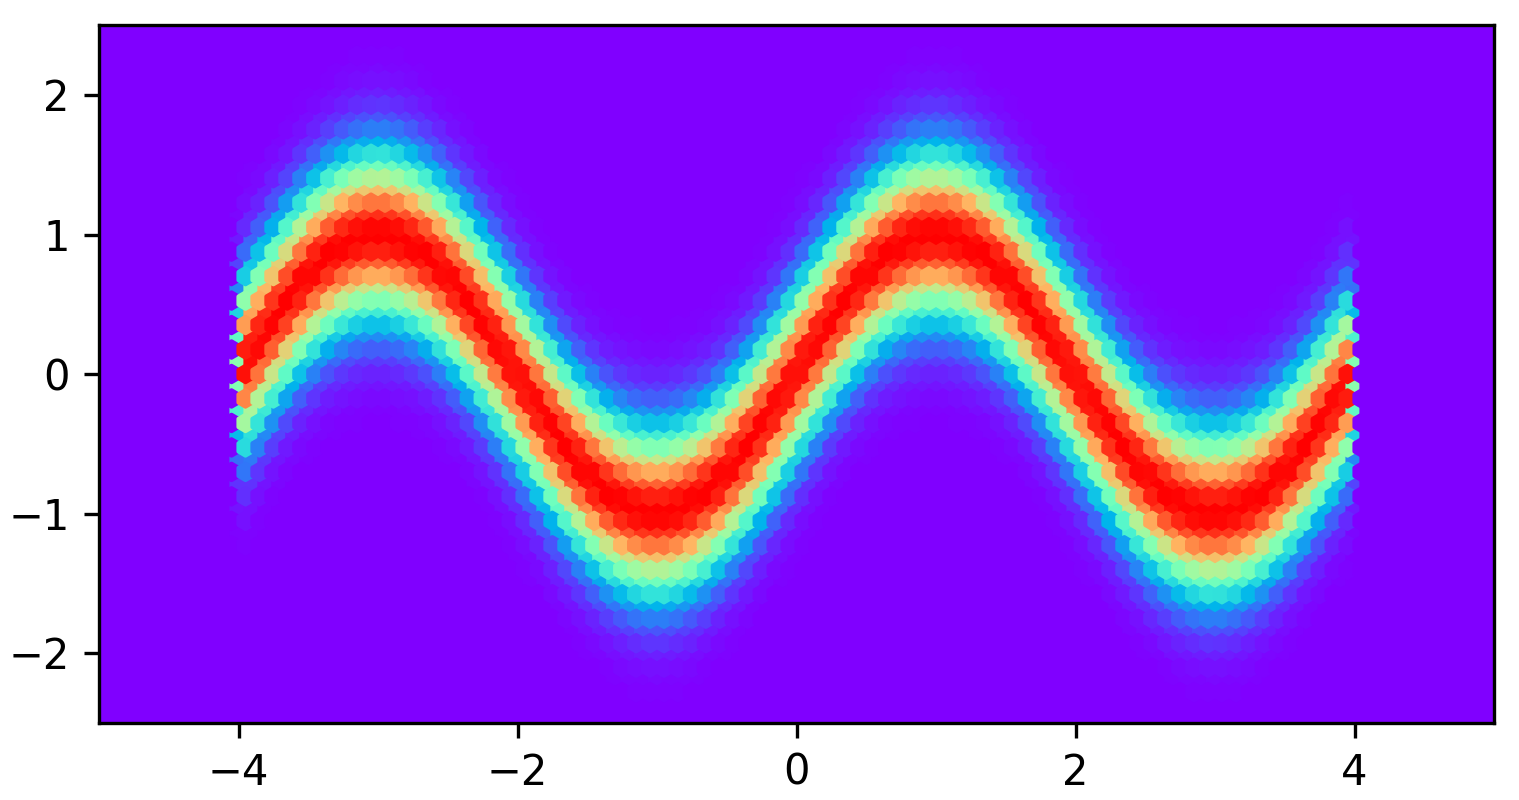
\includegraphics[width=0.5\textwidth]{example2-density}}
	\subfloat[Samples from Density 2]{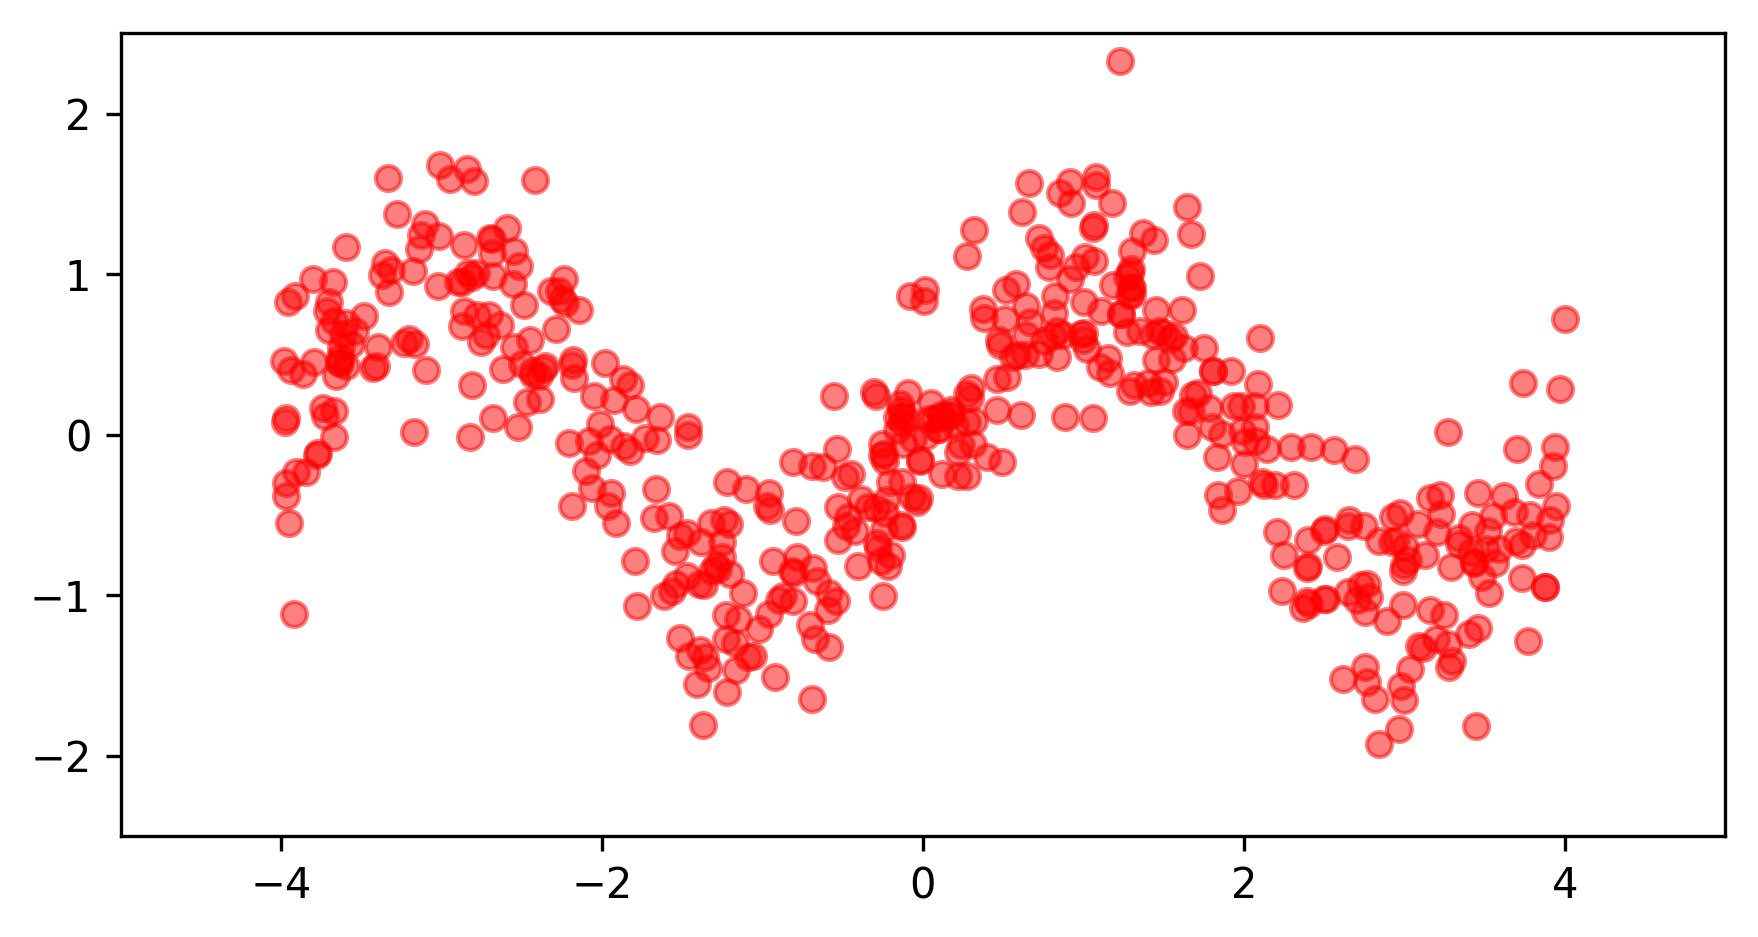
\includegraphics[width=0.5\textwidth]{example2-samples}}\\
	\caption{Two probability densities and samples from each density obtained using Metropolis-Hastings}
	\label{fig:densities}
\end{figure}

\begin{figure}
	\centering
	\subfloat[K = 2]{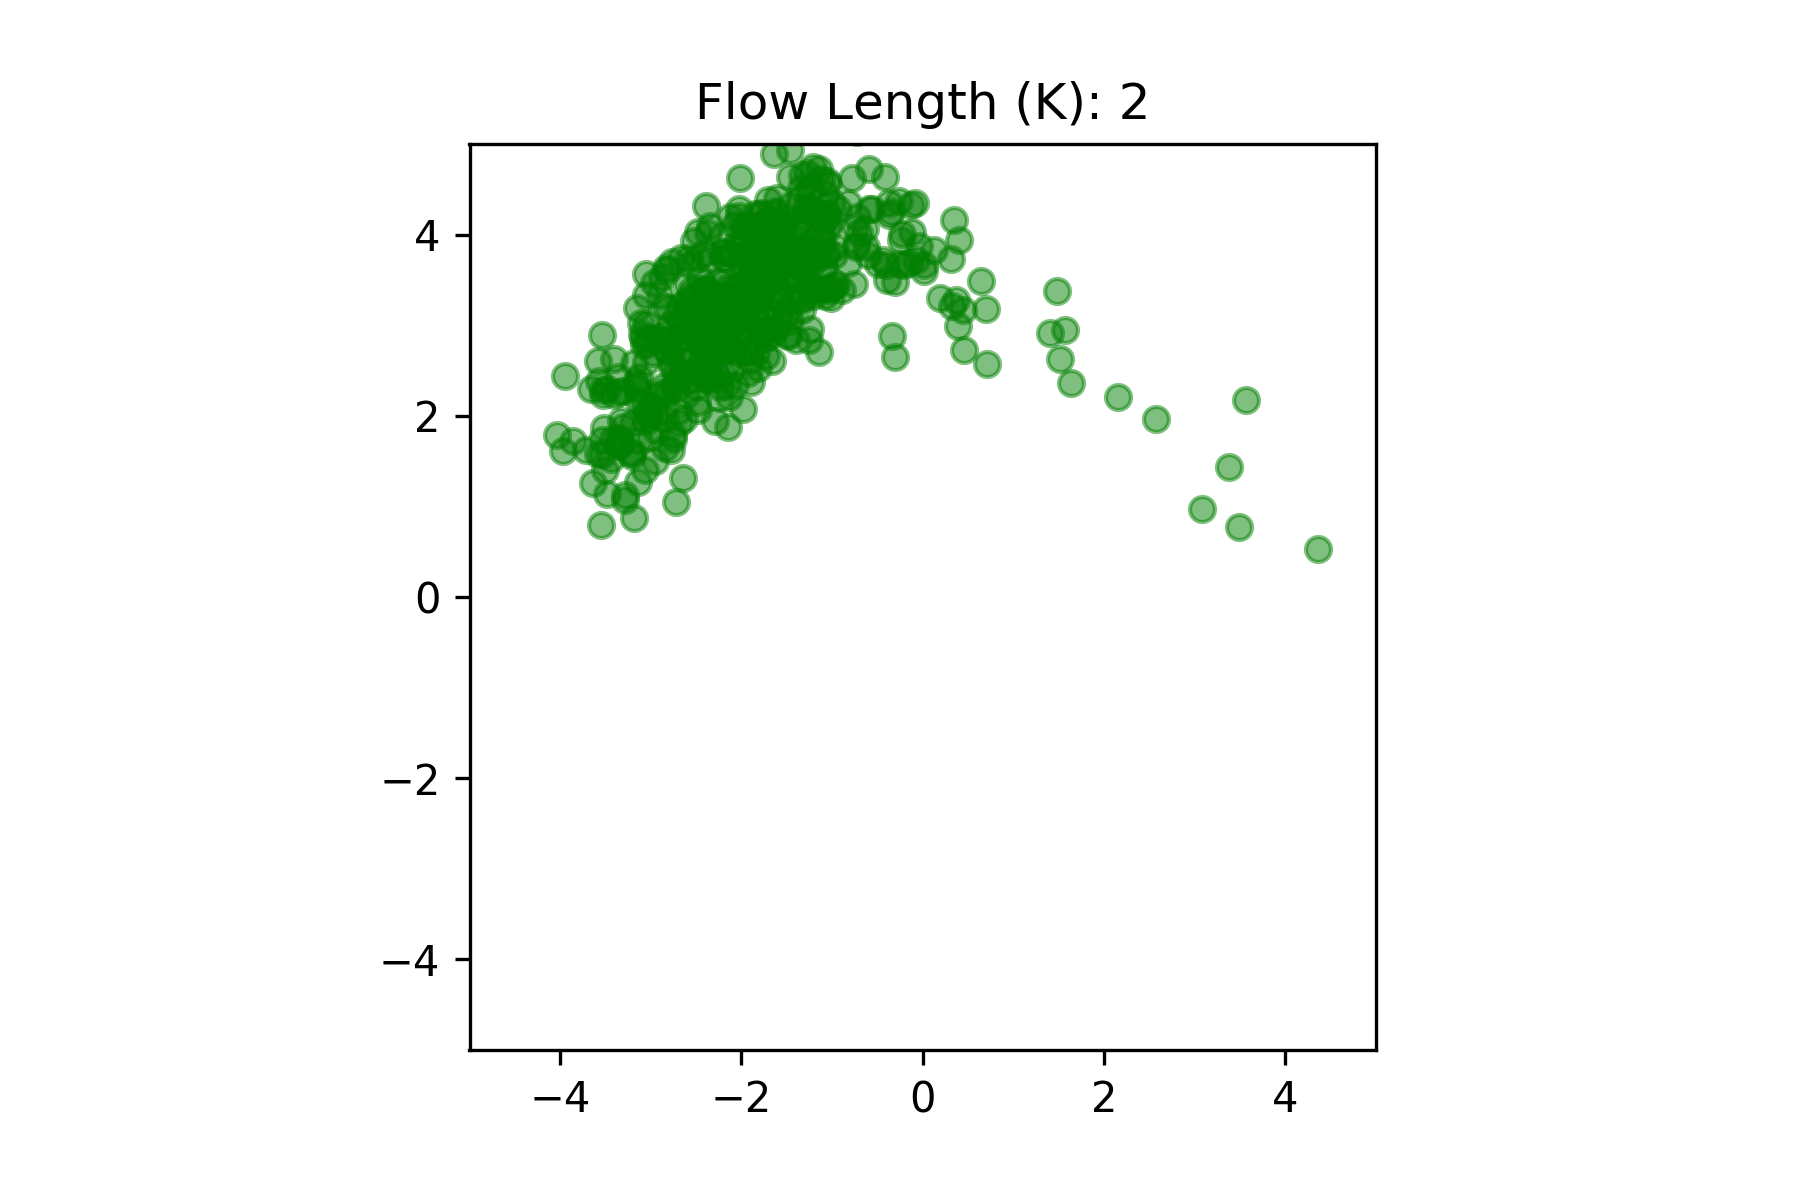
\includegraphics[width=0.5\textwidth]{example1-k2}}
	\subfloat[K = 4]{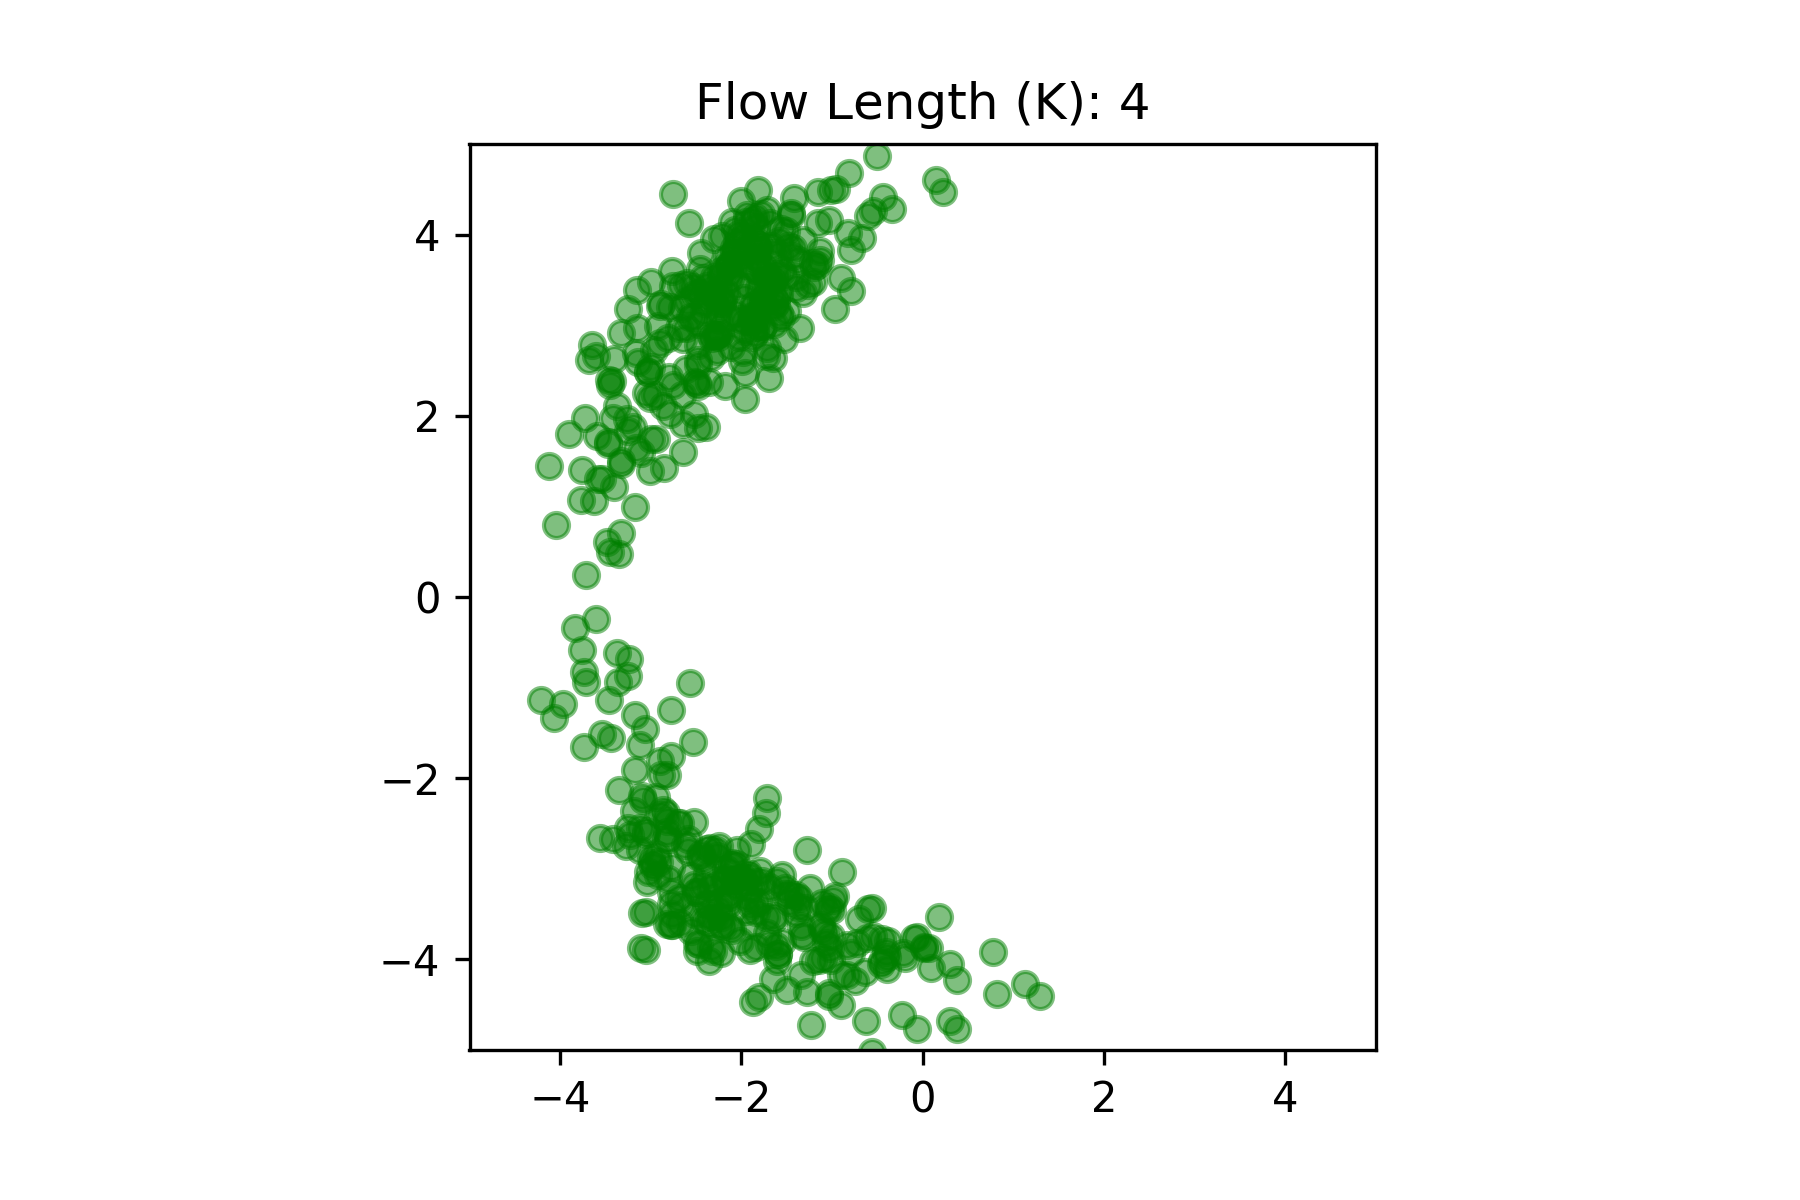
\includegraphics[width=0.5\textwidth]{example1-k4}}\\
	\subfloat[K = 8]{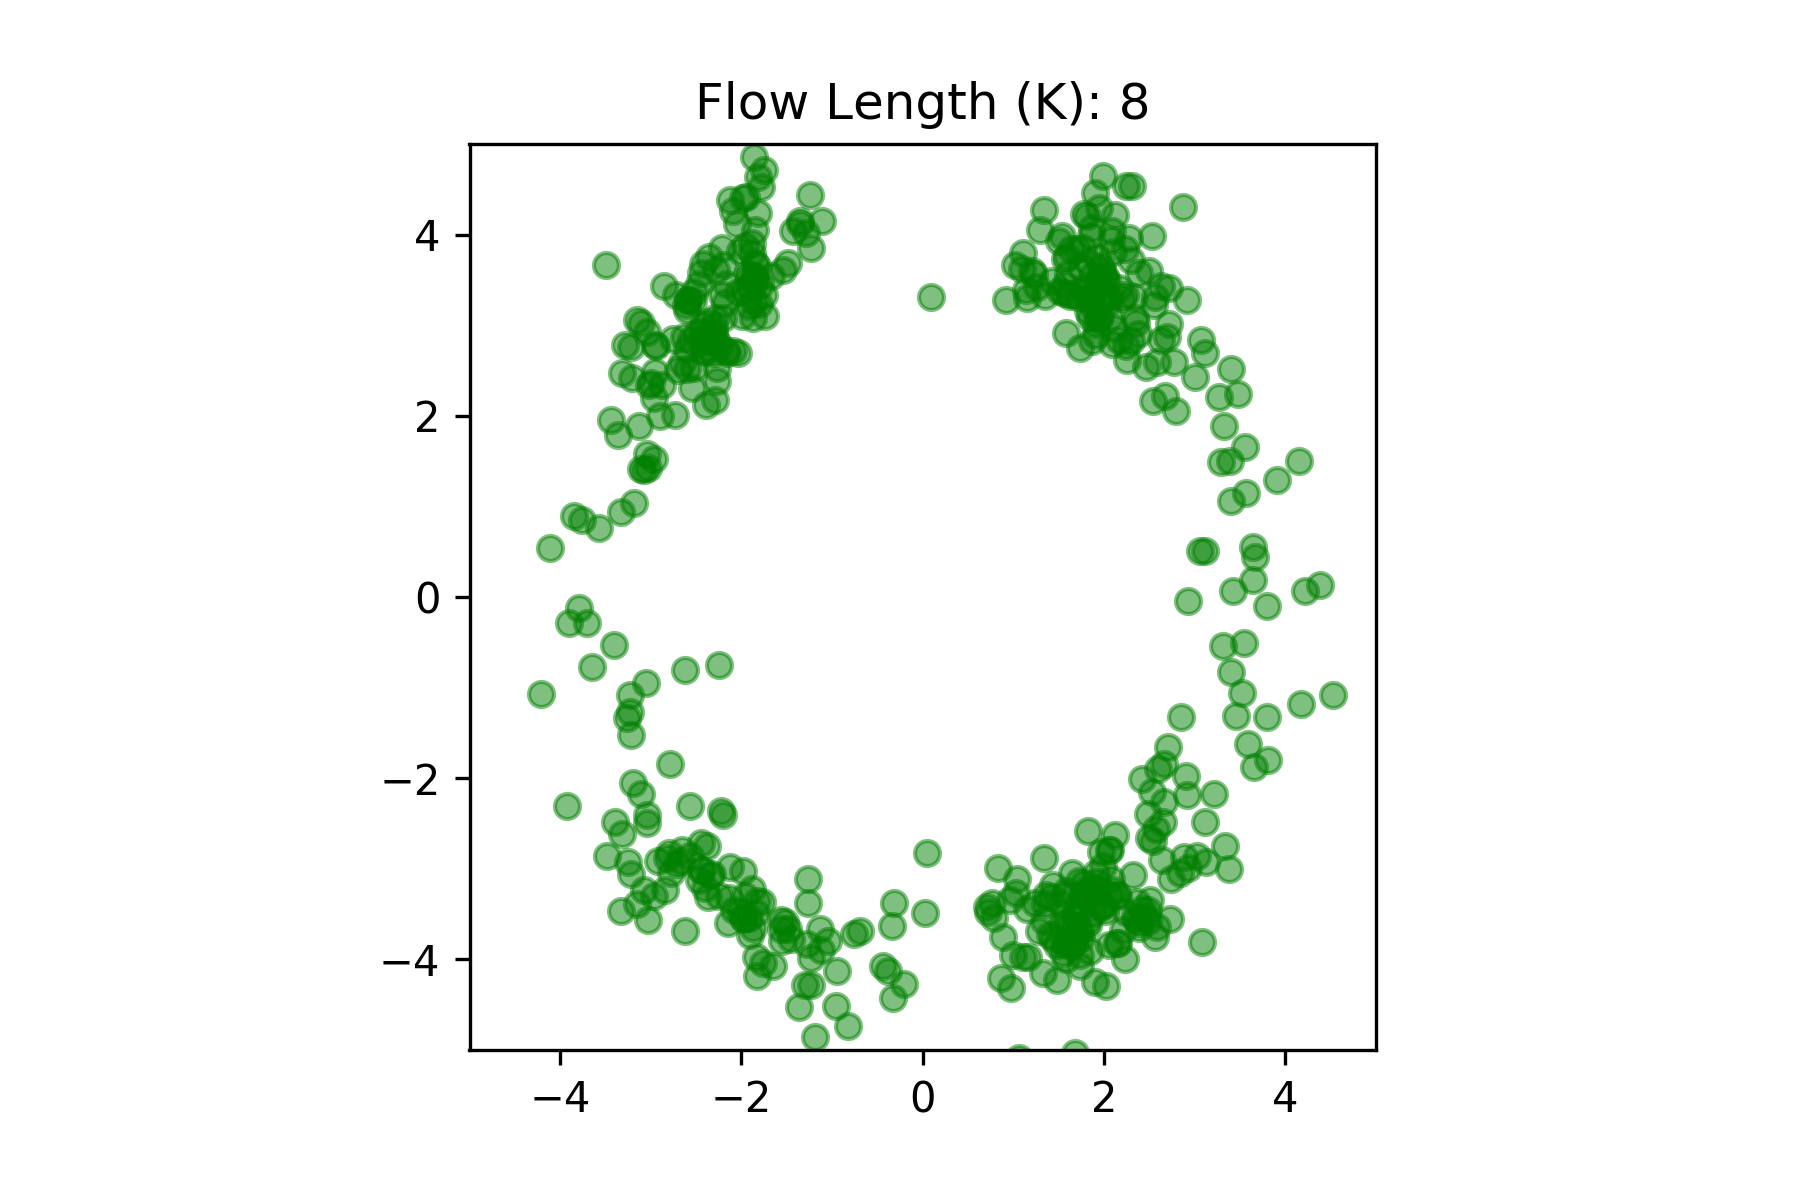
\includegraphics[width=0.5\textwidth]{example1-k8}}
	\subfloat[K = 16]{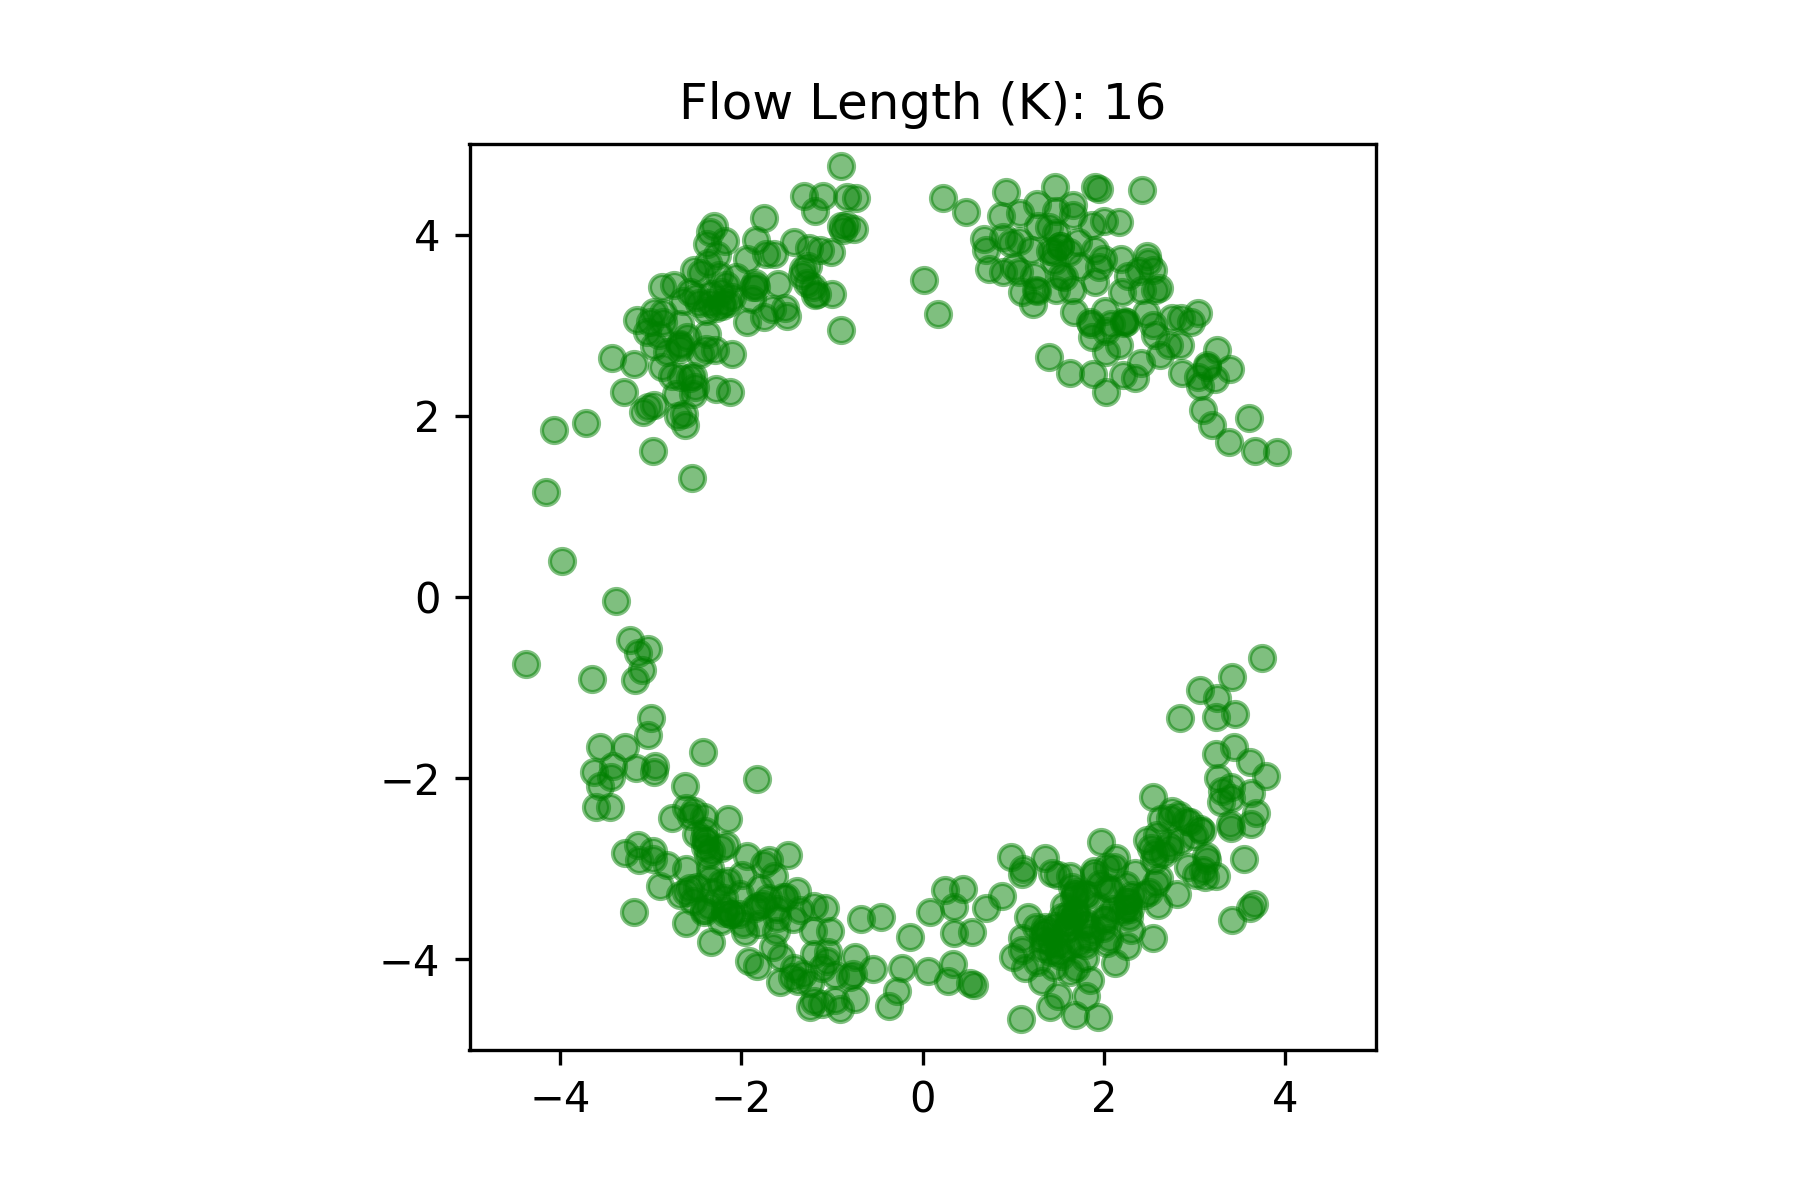
\includegraphics[width=0.5\textwidth]{example1-k16}}\\
	\caption{500 samples from Planar Flows with different flow lengths after 10000 training steps for density 1}
	\label{fig:density1}
\end{figure}

\begin{figure}
	\centering
	\subfloat[K = 2]{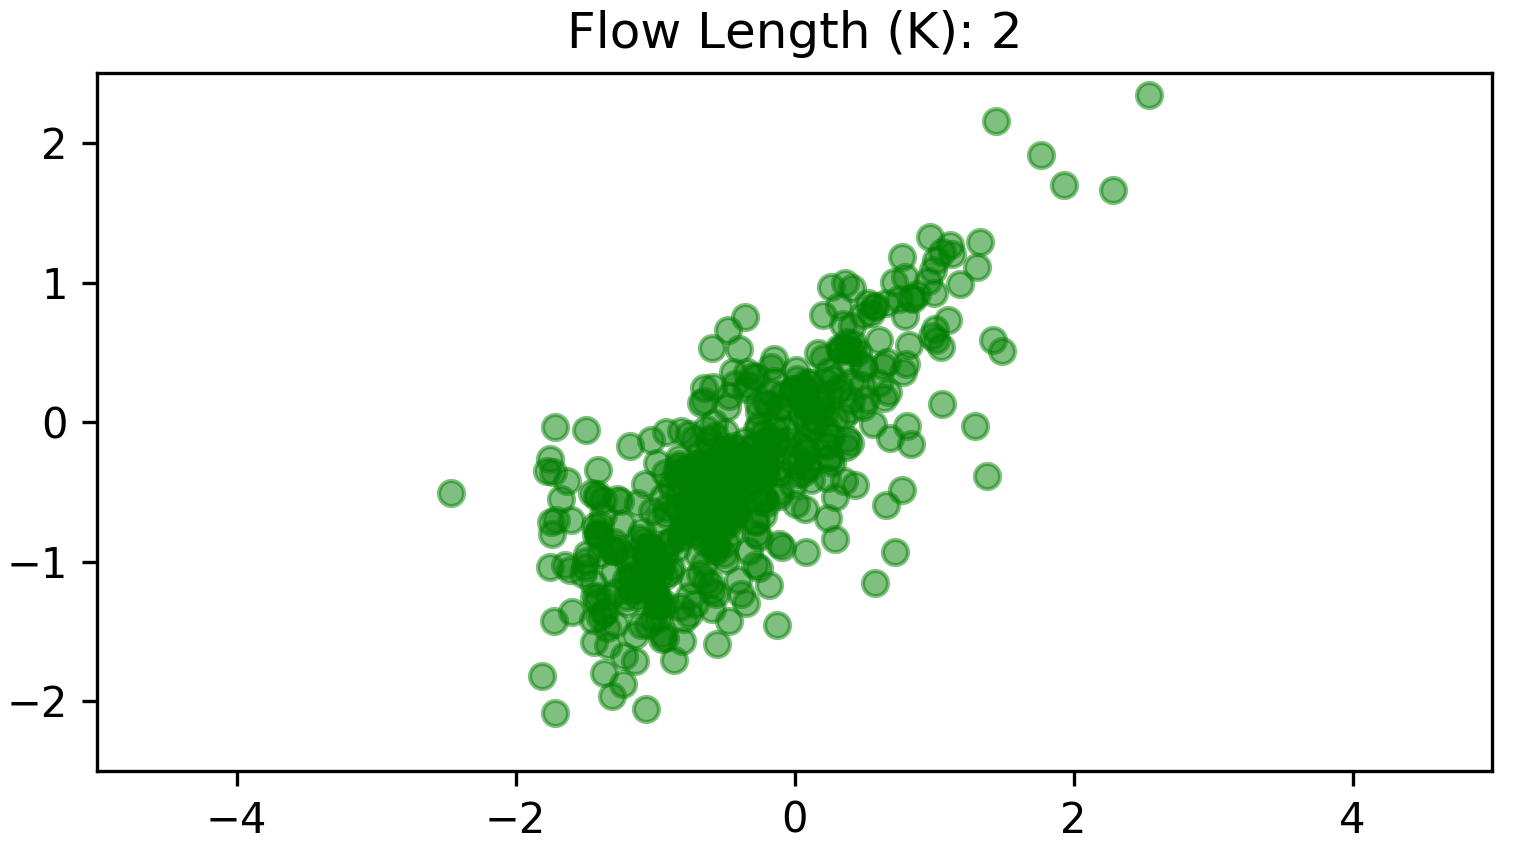
\includegraphics[width=0.5\textwidth]{example2-k2}}
	\subfloat[K = 4]{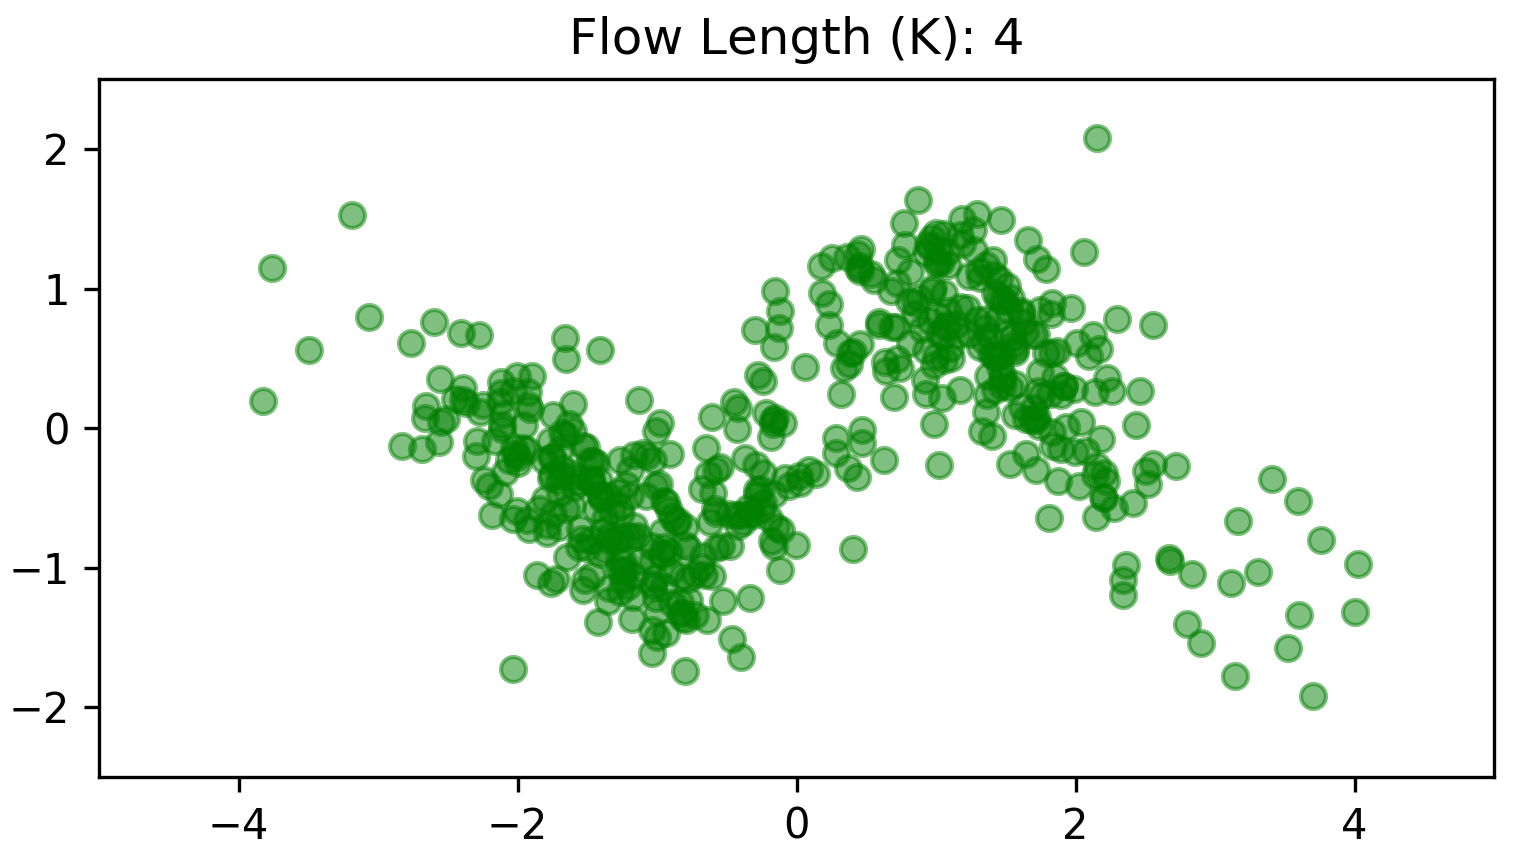
\includegraphics[width=0.5\textwidth]{example2-k4}}\\
	\subfloat[K = 8]{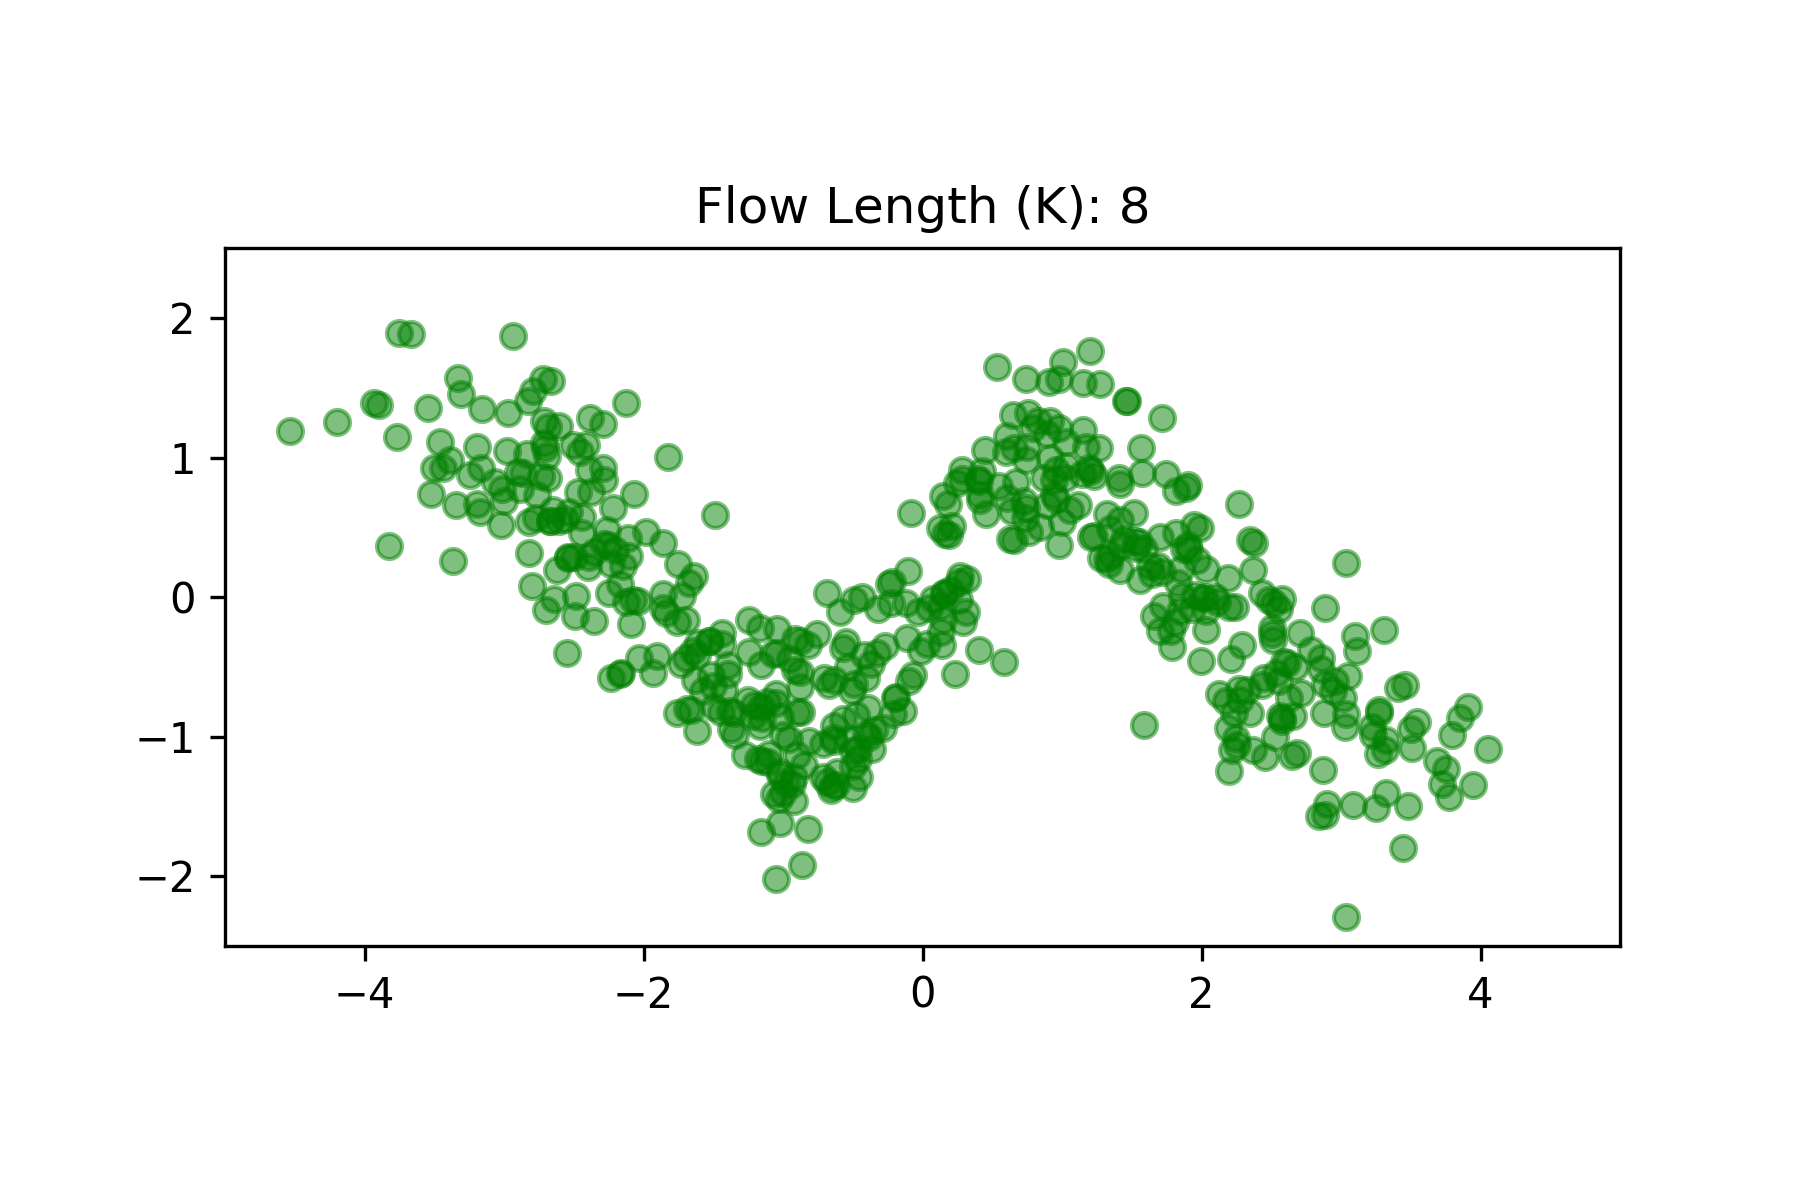
\includegraphics[width=0.5\textwidth]{example2-k8}}
	\subfloat[K = 16]{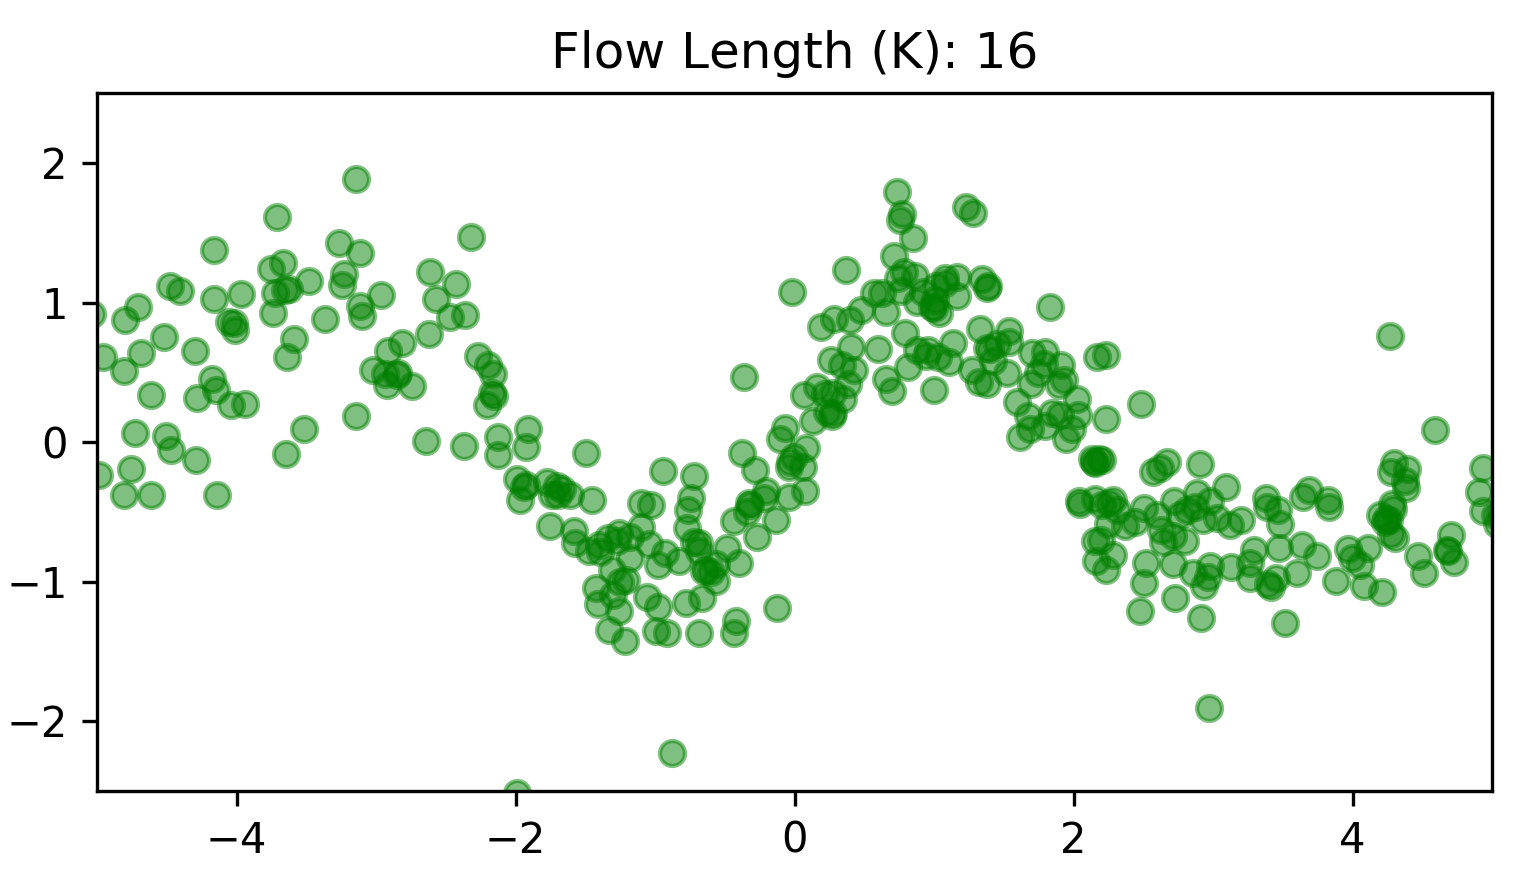
\includegraphics[width=0.5\textwidth]{example2-k16}}\\
	\caption{500 samples from Planar Flows with different flow lengths after 5000 training steps for density 2}
	\label{fig:density2}
\end{figure}

Fig. \ref{fig:densities} shows the two densities along with a scatter plot of 500 samples from each density obtained using Metropolis-Hastings (MH) algorithm. The MH algorithm was implemented in \texttt{numpy} using the normal distribution with identity covariance matrix as the proposal distribution. A part of the code that implements the MH algorithm is given in Snippet \ref{code:mh}. See \texttt{Metropolis-Hastings.ipynb} for complete code.

Planar Flow was implemented in Tensorflow and the code satisfies the invertibility conditions mentioned in the appendix of CITE. Tensorflow Probability (TFP) was not used because it requires implementation of the \texttt{\_inverse} function which is not available for the function used in planar flows although they are invertible. Flow lengths ($K$) from the set $\{2, 4, 8, 16\}$ were tested and trained using the Adam optimizer. A part of the code that implements planar flow is given in Snippet \ref{code:planar}. See \texttt{PlanarFlow-Example1.ipynb} and \texttt{PlanarFlow-Example2.ipynb} for complete code. Note that constant terms were dropped during the computation of the KL-divergence which may lead to negative KL values.

Figs. \ref{fig:density1} and \ref{fig:density2} show samples from planar flows of different lengths for density 1 and density 2 respectively at the end of training. It is clear from the results that as flow length increases, the model is able to better approximate the true density. Another interesting aspect encountered during the course of experiments was that the training becomes unstable as length of flow $K$ increases, especially for density 2. 

\begin{code}
	\inputminted[linenos=true,frame=lines,framesep=2mm]{python}{metropolis.py}
	\captionof{listing}{Metropolis-Hastings}
	\label{code:mh}
\end{code}
\begin{code}
	\inputminted[linenos=true,frame=lines,framesep=2mm]{python}{planar.py}
	\captionof{listing}{Planar Flow}
	\label{code:planar}
\end{code}

\end{document}